

\documentclass[../../e3_tp2_main.tex]{subfiles}

\begin{document}
\section{Ejercicio 6}

Se implementaron un latch SR y un flip flop D a partir de compuertas lógicas discretas. En ambos casos, se midieron sus parámetros característicos, y se compararon los resultados obtenidos con de sus equivalentes comerciales.
\subsection{Flip flop D}
\subsubsection{Funcionamiento}
El flip flop tipo D transfiere la entrada a la salida en cada ciclo de \textit{clock}. Por ende, se lo puede utilizar como unidad básica de memoria.
\begin{figure}[H]	
	\centering
	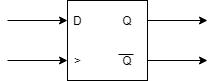
\includegraphics[width=0.3\textwidth]{imagenes/ffd_b.png}
	\caption{Representaci\'on del flip flop}
\end{figure}

\begin{table}[H]
\begin{center}
\begin{tabular}{|c|c|c|}
\hline
clk& D & Q\\
\hline \hline
$\uparrow$ & X & X \\ \hline
$\downarrow$ &X  &$Q_{n-1}$ \\ \hline
\end{tabular}
\caption{Tabla de verdad del flip flop D} 
\end{center}
\end{table}

\subsubsection{Circuito lógico}
Una posible implementación del flip flop D es la siguiente:
\begin{figure}[H]	
	\centering
	
\includegraphics[width=0.5\textwidth]{imagenes/ffd_cd.png}
	\caption{Circuito digital del flip flop D}
\end{figure}
\subsubsection{Implementación y medici\'on}
Se implementó el circuito indicado en la sección anterior con compuertas lógicas \textit{nand}. Para ello, se utilizó el integrado 74HC00.\par

Del circuito previamente mencionado, se midió el tiempo de establecimiento, el \textit{rise time} y el \textit{fall time}. 

\begin{table}[H]
\begin{center}
\begin{tabular}{|c|c|c|c|c|}
\hline
clk& D & $Q_{n-1}$ & $Q_n$ &Tiempo de establecimiento\\
\hline \hline
$\uparrow$ &0& 1&0&$25.2 n s$  \\ \hline
$\uparrow$ &1&0&1&$29 n s$  \\ \hline
\end{tabular}
\caption{Tiempo de establecimiento del flip flop D medido} 
\end{center}
\end{table}

\begin{table}[H]
\begin{center}
\begin{tabular}{|c|c|}
\hline
Rise time& Fall time \\
\hline \hline
$45 n s$  & $49.6 n s$ \\ \hline
\end{tabular}
\caption{Rise time y fall time medidos para el flip flop D.} 
\end{center}
\end{table}

Para realizar la comparación se eligió el integrado comercial 74HC74. De su hoja de datos\footnote{Disponible en: \url{http://www.mouser.com/ds/2/308/74HC74-108792.pdf} (consultado: 14/10/2018).}, se obtuvieron los siguientes tiempos:

\begin{table}[H]
\begin{center}
\begin{tabular}{|c|c|c|c|c|}
\hline
clk& D & $Q_{n-1}$ & $Q_n$ &Tiempo de establecimiento\\
\hline \hline
$\uparrow$ &0& 1&0&$13 n s$  \\ \hline
$\uparrow$ &1&0&1&$18 n s$  \\ \hline
\end{tabular}
\caption{Tiempo de establecimiento del 74HC74 seg\'un su \textit{data sheet}} 
\end{center}
\end{table}

\begin{table}[H]
\begin{center}
\begin{tabular}{|c|c|}
\hline
Rise time& Fall time \\
\hline \hline
$<400 n s$  & $<400 n s$ \\ \hline
\end{tabular}
\caption{Rise time y fall time del 74HC74 seg\'un su \textit{data sheet}} 
\end{center}
\end{table}

Como se puede observar, los tiempos de propagación del flip flop comercial son menores a los del que se implementó. Esto se puede deber a que el comercial hace un uso m\'as eficiente de los transistores.

\subsection{Latch SR}

\subsubsection{Funcionamiento}
El latch SR posee tres entradas: una de \textit{clock}, para poder sincronizar, otra de set (pone la salida a \textit{high}) y de reset (salida en \textit{low}).
\begin{figure}[H]	
	\centering
	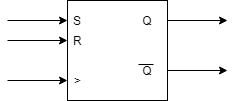
\includegraphics[width=0.2\textwidth]{imagenes/lsr_b.png}
	\caption{Representaci\'on de un latch}
\end{figure}

\begin{table}[H]
\begin{center}
\begin{tabular}{|c|c|c|c|}
\hline
clk&S & R & Q\\
\hline \hline
$\uparrow$ & 0 & 0 & $Q_{n-1}$ \\ \hline
$\uparrow$ & 0 & 1 &0 \\ \hline
$\uparrow$ & 1 & 0 & 1 \\ \hline
$\uparrow$ & 1 &1 & Indeterminado \\ \hline

\end{tabular}
\caption{Tabla de verdad latch  SR} 
\end{center}
\end{table}

\subsubsection{Circuito lógico}
Una posible implementación del latch SR es la siguiente:
\begin{figure}[H]	
	\centering
	
\includegraphics[width=0.5\textwidth]{imagenes/lsr_cd.png}
	\caption{Circuito digital del latch SR}
\end{figure}

\subsubsection{Implementación y medici\'on}
Se implementó el circuito indicado en la sección anterior exclusivamente con compuertas lógicas \textit{nand}, reemplazando las \textit{nor} por un equivalente l\'ogico con este tipo de compuerta. Se volvi\'o a hacer uso, entonces, del integrado 74HC00.\par

Nuevamente, se midieron el tiempo de establecimiento, el rise time y el fall time. 

\begin{table}[H]
\begin{center}
\begin{tabular}{|c|c|c|c|c|c|}
\hline
clk& R&S & $Q_{n-1}$ & $Q_n$ &Tiempo de establecimiento\\
\hline \hline
$\uparrow$ &0 & 1 &0&1&$21.6 n s$  \\ \hline
$\uparrow$ &1 & 0 &1&0&$14 n s$  \\ \hline

\end{tabular}
\caption{Tiempo de establecimiento medido del latch SR} 
\end{center}
\end{table}

\begin{table}[H]
\begin{center}
\begin{tabular}{|c|c|}
\hline
Rise time& Fall time \\
\hline \hline
$21.6 n s$  & $14 n s$ \\ \hline
\end{tabular}
\caption{Rise time y fall time medidos del latch SR} 
\end{center}
\end{table}

Para realizar la comparación se eligió el integrado comercial 74HC279 de la hoja de datos\footnote{Disponible en: \url{http://noel.feld.cvut.cz/hw/st/1937.pdf} (consultado: 14/10/2018).}. Se obtuvieron los siguientes tiempos:

\begin{table}[H]
\begin{center}
\begin{tabular}{|c|c|c|c|c|}
\hline
clk& D & $Q_{n-1}$ & $Q_n$ &Tiempo de establecimiento\\
\hline \hline
$\uparrow$ &0& 1&0&$20n s$  \\ \hline
$\uparrow$ &1&0&1&$13 n s$  \\ \hline
\end{tabular}
\caption{Tiempo de establecimiento del 74HC279 seg\'un su \textit{data sheet}} 
\end{center}
\end{table}

\begin{table}[H]
\begin{center}
\begin{tabular}{|c|c|}
\hline
Rise time& Fall time \\
\hline \hline
$<400 n s$  & $<400 n s$ \\ \hline
\end{tabular}
\caption{Rise time y fall time del 74HC279 seg\'un su \textit{data sheet}} 
\end{center}
\end{table}





\end{document}
